\documentclass[11pt]{amsart}
\usepackage{geometry}                % See geometry.pdf to learn the layout options. There are lots.
\geometry{letterpaper}                   % ... or a4paper or a5paper or ... 
%\geometry{landscape}                % Activate for for rotated page geometry
%\usepackage[parfill]{parskip}    % Activate to begin paragraphs with an empty line rather than an indent
\usepackage{graphicx}
\usepackage{amssymb}
\usepackage{epstopdf}
\usepackage[usenames,dvipsnames]{color}
\usepackage{fancyvrb}
\usepackage{listings}
\usepackage{booktabs,footmisc}
\usepackage{hyperref}
\usepackage[all]{hypcap}

\usepackage{topcapt}


 
% include the lines below to use a nicer fixed-width font than the default one
 
\lstset{fancyvrb=true}
\lstset{
	basicstyle=\small\tt,
	identifierstyle=,
	commentstyle=\color{Bittersweet},
	stringstyle=\color{red},
	showstringspaces=false,
	tabsize=3,
	numbers=left,
	captionpos=b,
	xleftmargin=2em
%	numberstyle=\tiny
	%stepnumber=4
	}
\DeclareGraphicsRule{.tif}{png}{.png}{`convert #1 `dirname #1`/`basename #1 .tif`.png}

\title{Termites Model Description}
\author{Grace I. Lin - GSoC 2011}
%\date{\today}                                           % Activate to display a given date or no date

\begin{document} 
\maketitle

\tableofcontents 

\section{Model Description}
The termites model simulates termites pick up and drop off wood chips.  There are different ways to model such behavior, and this version works as follow.  The carrying of a chip is indicated by the termite's state: NO\_CHIP, HAS\_CHIP.  Each termite finds "empty sites" within its eight directions, counting locations with chip as empty sites as well.  It picks a random location from the list and tires to move there.  If the location contains a chip, and the termite already carries a chip, then drop the chip nearby.  If the termite does not carry a chip, then pick up the chip and move to the new location.  On the other hand, if the location really is empty (no chip), then simply move the termite to the new location.\\

Since initially all termites and chips are scattered randomly (Figure \ref{fig:termite_before}), we will see clusters of chips as time goes on (Figure \ref{fig:termite_after}).  Also note that since every termite can carry one chip, if the number of chips is less than the number of termites, then it is possible that no clusters will occur.  Depending on the ratio of chips to termites, we would see the forming of clusters at various time.  The larger the ratio, the slower the formation of clusters, as it takes more time for termites to move around all the chips.\\

The chip class is pretty much unused, but it is left in for possible expansions later.

\begin{figure}[h]
\begin{center}
\vspace{.2in}
\centerline {
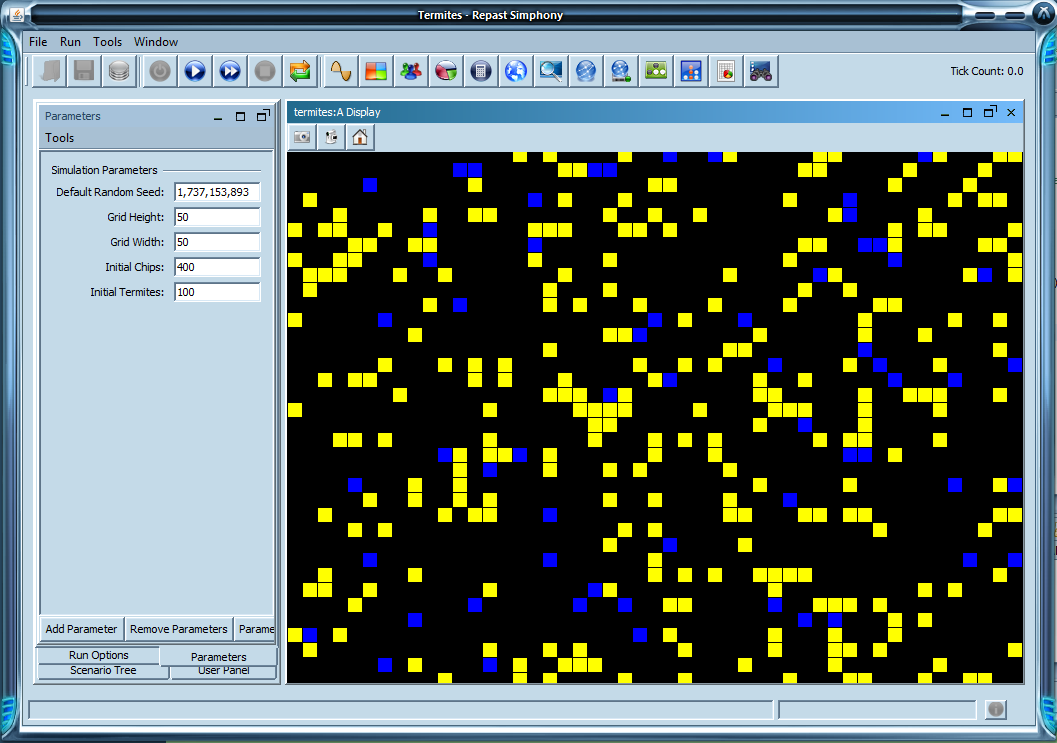
\includegraphics[width=5in]{Images/termite_before.png}}
\caption{Termites Model - at initialization}
\label{fig:termite_before}
\end{center}
\end{figure}

\begin{figure}[h]
\begin{center}
\vspace{.2in}
\centerline {
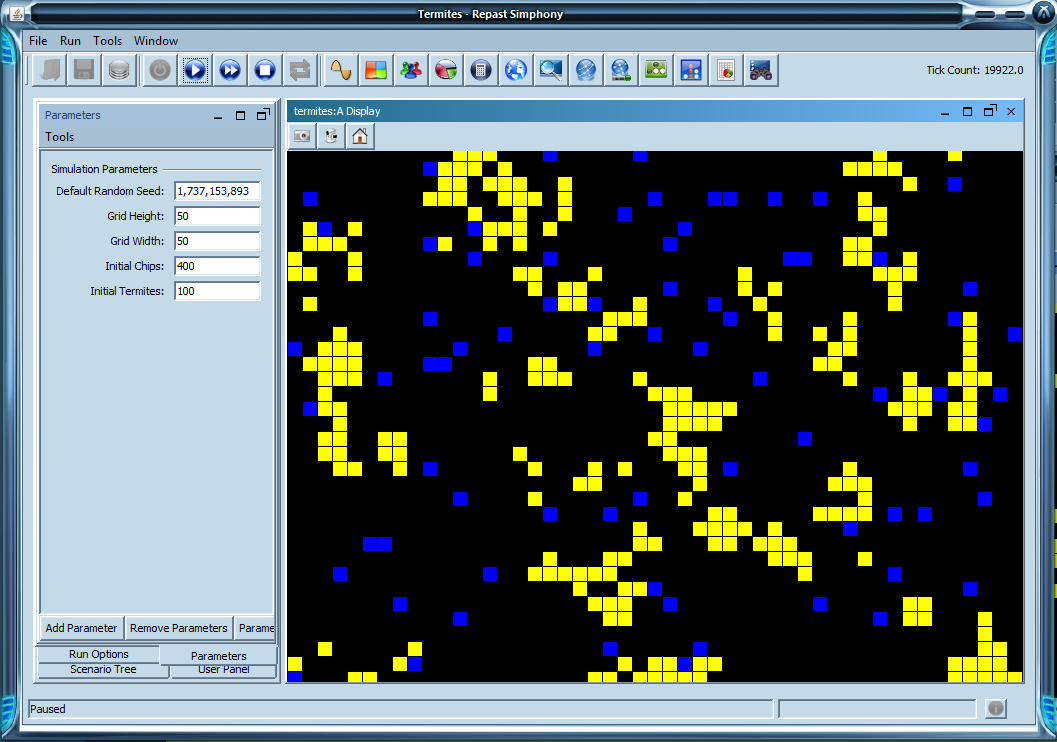
\includegraphics[width=5in]{Images/termite_after.png}}
\caption{Termites Model - after some time }
\label{fig:termite_after}
\end{center}
\end{figure}


\section{Model Parameters}

Termites are blue, and chips are yellow.  There are only a few parameters for the model: 

\begin{itemize}
\item Grid Height:  Number of rows.
\item Grid Width:  Number of columns.
\item Initial Chips:  Number of chips to populate initially.
\item Initial Termites:  Number of termites to populate initially.
\end{itemize}
\vspace{.2in}

\section {References}

\begin{itemize}
\item NetLogo's termites model: \emph{http://ccl.northwestern.edu/netlogo/models/Termites}
\end{itemize}

\end{document}  